\begin{problem}{Grid Reboot}{standard input}{standard output}{3 seconds}{512 megabytes}

You are managing a neural network consisting of $N$ terminals connected by $M$ bidirectional links. Each terminal is currently either offline (0) or online (1). Triggering a reboot signal on terminal $u$ toggles the state of terminal $u$ and all terminals directly connected to it (changing 0 to 1 and 1 to 0). You are given $Q$ independent emergency scenarios, each providing the initial state of all $N$ terminals. For each scenario, find a set of terminals to reboot so that all $N$ terminals end up online (1), or determine that it is impossible.

\InputFile
The first line contains three integers $N$, $M$, and $Q$ ($N, M \le 3000$, $Q \le 500$) --- the number of terminals, links, and emergency scenarios. The next $M$ lines each contain two 1-indexed integers $u$ and $v$ ($1 \le u, v \le N, u \neq v$), representing an undirected link between terminals $u$ and $v$. The next $Q$ lines each contain N characters of 0s and 1s, where the $i$-th character denotes the initial state of terminal $i$ (0 = off, 1 = on).

\OutputFile
For each scencarios, output a single line:


--- If it is impossible to make all terminals online, print -1.


--- Otherwise, print an integer $K$ ($0 \le K \le N$), followed by $K$ distinct space-separated 1-indexed integers indicating the chosen terminals to operate on. If there are multiple valid solutions, you may output any.

\Example

\begin{example}
\exmpfile{example.01}{example.01.a}%
\end{example}

\Note
Consider the second query; this is the initial state of all terminals in the network (let all bold vertices represent online terminals):


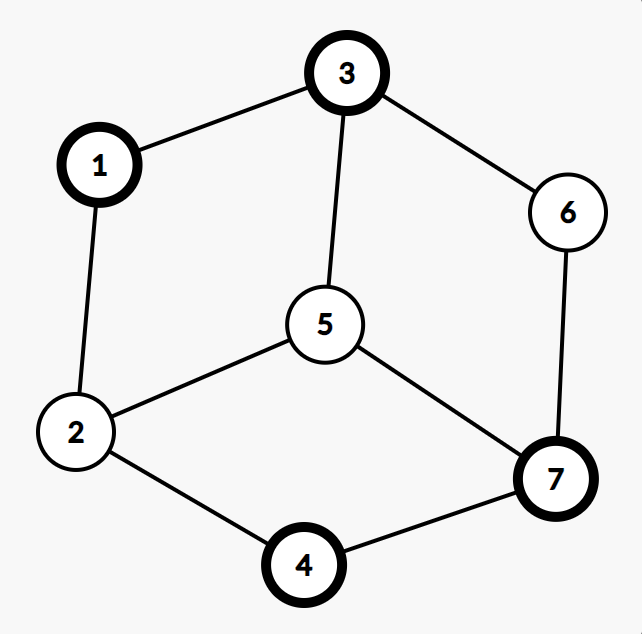
\includegraphics[width=10cm]{fig1.png}


Triggering a reboot signal on terminal 1:


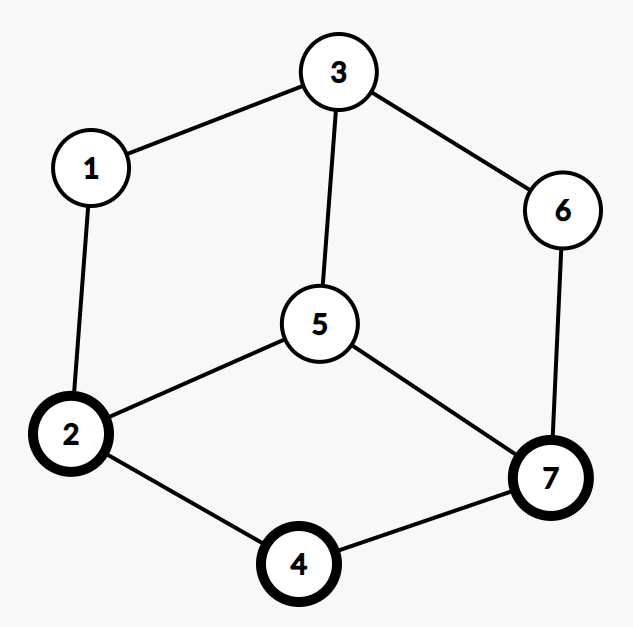
\includegraphics[width=10cm]{fig2.png}


Finally, triggering terminal 3 will result in the following state of the network:


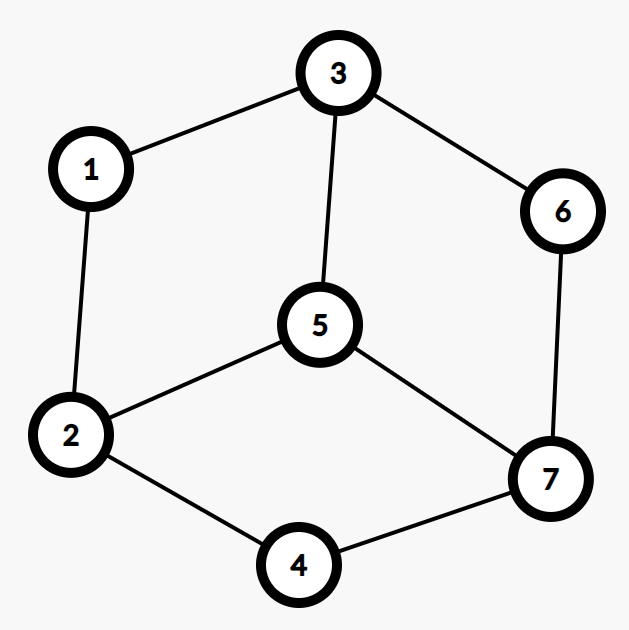
\includegraphics[width=10cm]{fig3.png}


Alternatively, you can trigger terminal 4 and 7 which also make all terminals online.

\end{problem}

